\documentclass[english, twocolumn]{article}
%%%%%%%%%%%%%%%%%%%%%%%%%%%%%%%%%%%%%%%%%%%%%%%%%%%%%%%%%%%%%%%%%%%%%%%%%%%%%%%%%%%%%%%%%%%%%%%%%%%%%%%%%%%%%%%%%%%%%%%%%%%%
\usepackage{latexsym,amsmath,amssymb,amsfonts,fullpage,graphicx, float}
\usepackage{lastpage}
\usepackage[hang, small,labelfont=bf,up,textfont=it,up]{caption} % Custom captions under/above floats in tables or figures
\usepackage{placeins}
\usepackage{adjustbox}
\usepackage[toc,page]{appendix}
\usepackage{tabulary}
\usepackage[margin=0.5in]{geometry}
\title{MEAM 620 Project 3} 
\author{Lou Lin, Mary Ibrahim, Gabrielle Merritt}
\begin{document}
\maketitle

\begin{abstract}
Included in this report are the details of our solution to Phase 4 of Project 1. The project required this team to draw on previous code submissions for Project 1 in MEAM620 that culminated with the implementation of a controller for a KMel Nano+ to follow a planned trajectory. The final phase consisted of 2 parts; a controller and a trajectory planner.  Our controller was adapted from code produced by Jay Davey in Project 1 Phase 2.  Our trajectory planner was adapted from code by Alex Burka and Gabrielle Merritt in Project 1 Phase 3.  Unknown waypoints were provided that the quadrotor had to navigate through.  This report details how our group was able to fly a micro aerial vehicle along the path we found through a list of unknown waypoints. 
\end{abstract}

\section*{Methods}
For this assignment we broke the work into two main sections, the first being the position controller for the quadrotor (attitude was handled on board the quadrotor), and generating smooth trajectories for the controller to follow. 
\subsection*{Controller}
\subsubsection*{PID architecture}

Our controller was designed with a linearized model of the quadrotor and a nested control structure.  The same controller was used for hovering, single waypoint navigation and multi waypoint navigation. A nested control structure was used so that the attitude controller could run at a faster rate (1kHz) than the position controller (100Hz).  Figure 1 shows a block diagram of our control architecture.
\nolinebreak
\begin{figure}[!h]
\caption{Controller Architecture}
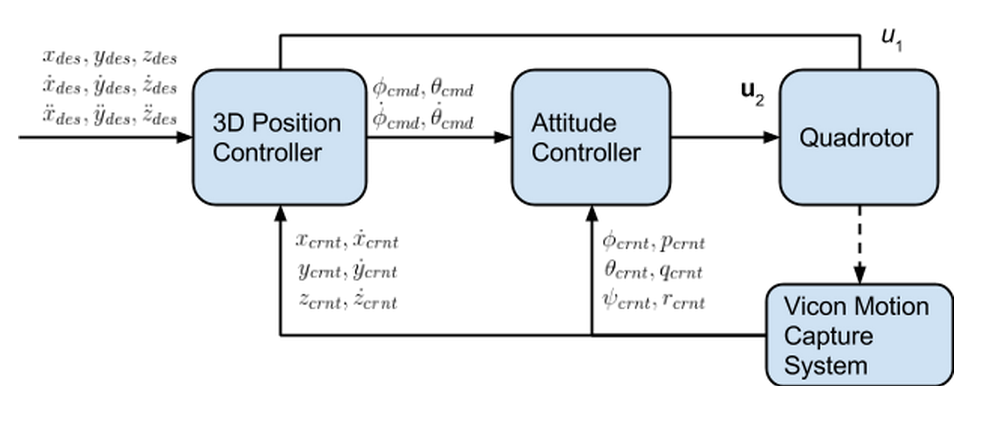
\includegraphics[width = \linewidth]{PID.png}
\end{figure}
\FloatBarrier
\subsubsection*{Equations for Control}
 First we obtained the error between the desired angular and linear positions and velocities 
\begin{table}[ht]
\resizebox{.5\textwidth}{!}{\begin{tabular}{llll}
Linear Position Error        & Angular Position Error & Linear Velocity Error                          & Angular Velocity Error \\
$e_{x} = x_{des} - x_{crnt}$ &$ e_{\phi} = \phi_{des} - \phi_{crnt}$& $\dot{e_{x}} = \dot{x_{des}} - \dot{x_{crnt}}$ & $e_{p} = p_{des} - p_{crnt}$     \\
$e_{y} = y_{des} - y_{crnt}$ & $ e_{\theta} = \theta_{des} - \theta{crnt}$ & $\dot{e_{y}} = \dot{y_{des}} - \dot{y_{crnt}}$     & $e_{q} = q_{des} - q_{crnt}   $     \\

$e_{z} = z_{des} - z_{crnt}$ & $ e_{\psi} = \psi_{des} - \psi_{crnt}$   & $\dot{e_{z}} = \dot{z_{des}} - \dot{z_{crnt}}$        & $e_{r} = r_{des} - r_{crnt}$           
\end{tabular}}
\end{table} 
\FloatBarrier 
Using the error between desired and actual position we calculated which positions and velocities should be commanded to the motors.
\subsubsection*{Gains}
 After testing a variety of the gains we found that the suggested gains in the lab manual worked well for our system.
\begin{table}[ht]
\resizebox{.5\textwidth}{!}{\begin{tabular}{llllll} 
X Gains & Y Gains & Z Gains &$ \phi$ Gains & $\theta$ Gains & $\psi$ Gains \\
$K_{p,x} = 10$  &$ K_{p,y} = 10 $& $K_{p,z} = 15 $ & $K_{p,\phi} = 1.6$ & $K_{p,\theta} = 1.6$ & $K_{p,\psi} = 1$ \\
$K_{d,x} = 5$  & $K_{d,y} = 5$  & $K_{d,z} = 7$&  $K_{d,\phi} = .1$ & $K_{d,\theta} = .1$ & $K_{d,\psi} = 0$
\end{tabular}}
\end{table}
\FloatBarrier
\paragraph{Commanded Positions } 
$$\phi_{cmd} =   \frac{1}{g} \ddot{x}_{cmd} \sin(\psi_{crnt}) - \ddot{y}_{cmd}\cos(\psi_{crnt})$$
$$\theta_{cmd} =   \frac{1}{g} \ddot{x}_{cmd} \cos(\psi_{crnt}) + \ddot{y}_{cmd} \sin(\psi_{crnt})$$
$$\psi_{cmd} =   \psi_{des}$$
\paragraph{Commanded Accelerations}
$$\ddot{x}_{cmd} = \ddot{x}_{des} + K_{p,x} {e_{x}} + K_{d,x} {\dot{e_{x}}}$$
$$\ddot{y}_{cmd} = \ddot{y}_{des} + K_{p,y} {e_{y}} + K_{d,y} {\dot{e_{y}}}$$
$$\ddot{z}_{cmd} = \ddot{z}_{des} + K_{p,z} {e_{z}} + K_{d,z} {\dot{e_{z}}}$$ 

Since we assuming that the quadrotor's position will remain near hover we assume that \\
\begin{center}
$ p_{cmd} = 0 $ ,  $ q_{cmd} = 0$ ,  $r_{cmd} = \dot{\psi}_{des} $
\end{center}

\paragraph{Controller outputs }
$$u_1 = m(g + \ddot{z}_{cmd}) $$
$$u _2 = \left[ \begin{matrix} 
k_{p,\phi} e_{\phi} + k_{d,\phi} e_{p}\\
k_{p,\theta} e_{\theta} + k_{d,\theta} e_{q}\\
k_{p,\psi} e_{\psi} + k_{d,\psi} e_r\\
\end{matrix} \right]
$$
For thrust since the MRSL's communication architecture requires thrust in grams we scaled our thrust ($u_1$) by 1000:

$trpy = [1000u_1/g, \phi_{cmd}, \theta_{cmd}, \psi_{cmd}]$

$drpy = [0, 0, 0, 0]$
\subsubsection*{Controller limits}
All of the errors and quadrotor command values are internally limited by our controller, in an attempt to keep things near the linearization point and prevent a runaway robot.
\linebreak
\linebreak
Maximum error in x, y, z that goes into the controller equation:\\
 $e_x = 0.75 $ , $e_y =0.75$ ,  $e_z = 1.52$  \\
\linebreak
Maximum angle allowed for roll and pitch:\\
$\phi_{max} = 40 * \frac{\pi}{180}$ ,
$\theta_{max} = 40 * \frac{\pi}{180}$\\
\linebreak
Maximum overall thrust sent to quadrotor: \\ 
$F_{max} = 4mg$ ,
$F_{min} = .05mg$\\
\linebreak
Maximum moments sent to quadrotor:\\
$M_{xy, max} = 0.01$ ,
$M_{z, max} = 0.01$


\subsection*{Trajectory Generation}
 For generating most of the trajectories we used Gabby's trajectory generation algorithm. After eliminating straightaways on the path, the trajectory generator finds an appropriate amount of time each section of the path should take; this is done by taking the cube root of the distance between two successive points and scaling them by some constant (in this case 2) to ensure the quadrotor will not try to accelerate from point to point too quickly. After generating a vector of times for each segment of the path we fit a  quintic spline to generate a minimum jerk trajectory for each path segment.  
 \subsubsection*{Spline Generation for Helix }
 For the helix (See  Follow Waypoint Path 3), we used Alex's smoothing algorithm which first eliminated straight aways on the path leaving only the corners. This is done by taking a numerical second derivative of the path, and eliminating points with no curvature. Afterwards we used a quintic spline to generate a minimum jerk trajectory of points, velocities and accelerations near the corners of the path (stopping at each corner). After now having a more accurate mapping of the path, we interpolated a cubic spline, passing through only every 100th point of the minimum jerk trajectory, which gave a smooth trajectory, without stopping at every corner point. We only used this method on the helix path, since the other paths had relatively few points, or many corners that occur in quick succession.


\section*{Results and Discussion}
Our results indicate that our controller and trajectory planning code was able to fly the quadrotor through a given list of waypoints.  Some error can be observed in particular in the z-direction of the commanded trajectories.  This could have a few possible explanations.  In the lab manual documentation (page 3) there is a value for the z-offset that is set at 100mm.  There’s a possibility that this value might not be correct and instead should be closer to 148mm, which is 100mm  + 48mm our average error in the negative z-direction.  If the offset instead were 148mm then our average error could have been close to zero.  Instead, our average error was around 48mm over the course of the trajectories.  The maximum error with the 100mm offset was -78mm. If the offset were 148mm our maximum error would have been -30mm.  Other ways we could improve on the steady state error could include adding an integral term to the PD controller.  We also might not have had an optimally tuned $K_{p,z}$  gain (not high enough).  Another explanation could be that the value for the weight of the quadrotor could have been off but it is unlikely to have affected the controller by this amount of error observed. See graphs in appendix A. 

\section*{Conclusion} 

\section{\\Graphs} \label{App:AppendixA}


\end{document}
